\documentclass[../tesi.tex]{subfiles}
\begin{document}

\chapter{Casi di Studio}
\section{Apprendimento automatico nel campo delle Reti}

\newglossaryentry{Throughput}{
	name=Throughput,
	description=Quantitá di dati trasmessi in un unitá di tempo \textit{(Tasso di elaborazione o trasmissione)}
}

\newglossaryentry{CDN}{
	name=CDN,
	description={(\textit{Content Delivery Network}) Sistema di computer collegati in rete attraverso Internet, che collaborano in maniera trasparente sotto forma di sistema distribuito per ripartire contenuti e servizi agli utenti finali, riducendo anomalie dovute all'eccessivo numero di richieste al server principale}
}

\subsection{Panoramica}


Il Machine learning è un sottoinsieme delle AI, si sta sviluppando in ogni campo, nelle pagine seguenti andremo a studiare le opportunità usando il Machine Learning applicato alle reti.\\
L'Apprendimento automatico permette ai sistemi di imparare automaticamente e prendere decisioni o predizioni basati sull’esperienza.
Con lo sviluppo di internet, ricercatori e operatori di rete possono affrontare vari tipi di rete e applicazioni, le quali possono cambiare a seconda delle performance e dei requisiti.\\
L’incorporazione di ML nella gestione e nella pianificazione delle reti permette la possibilità di sviluppare nuove applicazioni di rete.\\
Il ML nelle reti può giocare un ruolo importante soprattutto nei problemi di reti più comuni, basti pensare a Intrusion Detection e Performance Prediction, inoltre è anche possibile aiutare a prendere decisioni facilitando lo scheduling di rete e l’adattamento di parametri in accordo con lo stato corrente dell’ambiente.\\
Altri problemi di rete invece, più complicati, hanno bisogno di interagire con sistemi complessi di rete, quali costruire e analizzare modelli che rappresentano sistemi complessi come il cambiamento di modelli delle \Gls{CDN} e delle caratteristiche di \Gls{Throughput}.\\
Machine Learning può fornire una stima di un modello di un sistema con un’accuratezza accettabile.\\
Infine, ogni scenario di rete ha diverse caratteristiche e i ricercatori spesso hanno bisogno di risolvere problemi per ogni scenario in maniera indipendente.

\subsection{Workflow}

\begin{figure}[htbp]
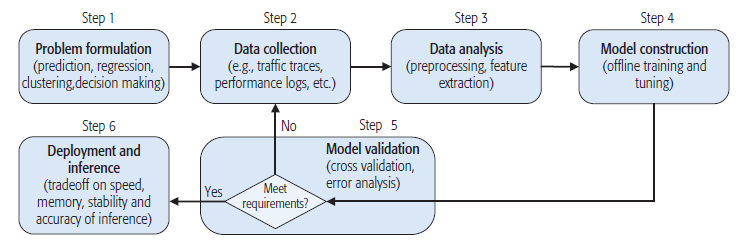
\includegraphics{WorkFlowNetworking.png}
\caption{ML Networking Workflow} 
\end{figure}

\newglossaryentry{over-fitting}{name={over-fitting},description={In presenza di un numero eccessivo di parametri rispetto al numero di osservazioni, un modello statistico si adatta ai dati osservati. Nei casi in cui l'apprendimento é stato effettuato troppo a lungo o dove c'era uno scarso numero di esempi di allenamento, il modello potrebbe adattarsi a caratteristiche che sono specifiche solo del \textit{training set} ma che non hanno riscontro nel resto dei casi.}}
\newglossaryentry{under-fitting}{name={under-fitting},description={Scenario che si presenta quando in un modello statisco o nell'algoritmo di ML non si riesce a catturare adeguatamente la struttura sottostante i dati. Si verifica quando il modello o l'algoritmo non si adattano abbastanza ai dati.La classificazione soffre di un'eccessiva discrepanza.(Il modello é troppo semplice)}}

\textit{Formulazione del problema}: Il processo di allenamento di ML spesso implica alti costi di tempo, è importante, dunque, formulare e astrarre correttamente il problema al primo step.\\
In questa fase ci si occupa di dividere il problema in una delle Categorie ML: Classificazione, Raggruppamento o Decisionali.
Questo ci aiuta a decidere che tipo e che mole di dati ci serve per il modello.\\
Un'astrazione impropria del problema può fornire un modello di apprendimento inadatto, che può risultare in prestazioni di apprendimento insoddisfacenti.\\
\\
\textit{Collezioni Dati}: In questa fase l’obiettivo è raccogliere un grande numero di dati rappresentativi senza bias, i dati di rete vengono raccolti da diversi livelli di rete in  accordo con l’applicazione di monitoraggio. Per esempio i problemi di classificazione del traffico  richiedono dataset contenti tracce a livello di pacchetto corrispondenti alle classi di applicazioni.\\
Nel contesto del MLN i dati sono spesso collezionati in due fasi.
Nella fase Offline, si raccolgono dati storici di alta-qualità importanti per le analisi e l’addestramento del modello mentre nella fase online si utilizzano dati dello stato di rete in real-time usati come input o come segnali di feedback per addestrare il modello.\\
\\
\textit{Analisi Dati}: Ogni problema di rete ha le proprie caratteristiche ed è influenzato da molti fattori.\\ 
Nel nostro caso di MLN trovare le caratteristiche adeguate è la chiave per potenziare al meglio il nostro modello.
Fondamentale in questa fase elaborare i dati grezzi attraverso processi di normalizzazione, discretizzazione e completamento del valore mancante, questa fase richiede una conoscenza specifica del dominio, in seguito si punterà ad estrarre le funzionalità effettive che possiamo trarre da questi dati.\\
\\
\textit{Costruzione Modello}: la costruzione del modello include la selezione e l’allenamento dello stesso. 
Un adatto modello di apprendimento o algoritmo ha bisogno di dati e dimensioni di essi il più coerenti possibili con le caratteristiche dello scenario di rete e la categoria del problema.\\
\\
\textit{Validazione del modello}: Validazione offline è uno step fondamentale nel workflow del MLN per valutare l’algoritmo di apprendimento. La convalida incrociata è spesso usata per testare l’accuratezza del modello(se il modello è over-fitting o \Gls{under-fitting}).
Questo prevede una buona guida su come ottimizzare il modello(e.g. aumentando il volume dei dati o riducendo la complessità del modello in caso questo sia \Gls{over-fitting})\\
\\
\textit{Deployment and Inference}: Quando implementiamo un modello di apprendimento automatico nell’ambiente di rete dobbiamo considerare alcuni problemi, ci possono essere limitazioni sulle computazioni o nelle risorse, bisogna trovare un tradeoff tra accuratezza e overhead per i sistemi pratici di reti. L’apprendimento automatico spesso funziona in best-effort e non fornisce alcune prestazioni di garanzia però bisogna comunque tener conto della tolleranza degli errori.
\subsection{Campi di Ricerca}
Parlando di apprendimento automatico possiamo già separare i case study in 3 categorie:\\
\begin{figure}[htbp]
\center
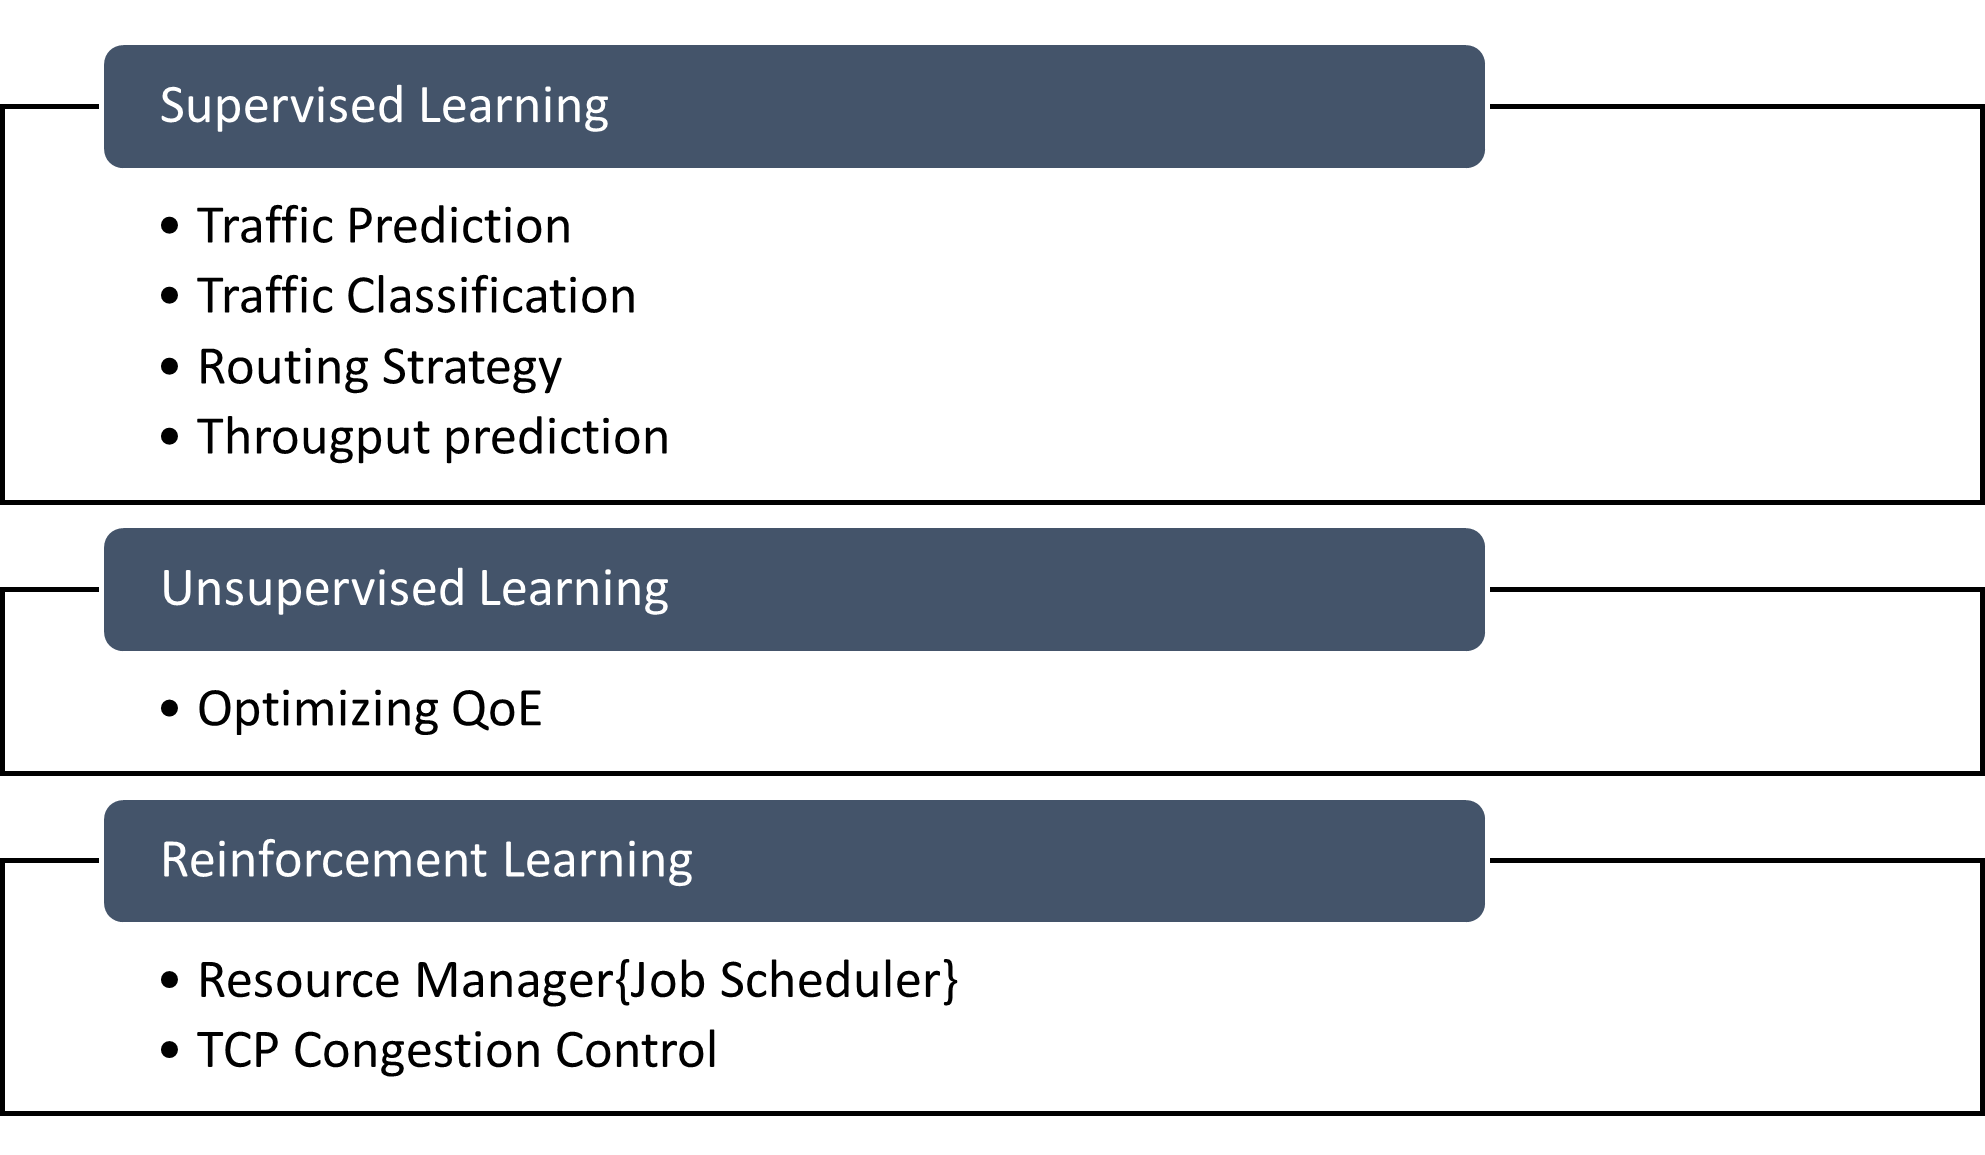
\includegraphics{RicercaMLNetworking.png}
\caption{} 
\end{figure}
\\
\newglossaryentry{port-based}{name={port-based},description={tecnica di classificazione basata sull'associazione $porta/protocollo$}}
\newglossaryentry{payload-based}{name={payload-based},description={tecnica di classificazione basata sul contenuto del pacchetto, associazione $contenuto/protocollo$}}
\newglossaryentry{Deep Learning}{name={Deep Learning},description={il Deep Learning é un campo di ricerca del ML che si basa su diversi livelli di rappresentazione.Intendiamo un insieme di reti neurali artificiali organizzate in diversi strati, dove ogni strato calcola i valori per quello successivo affinche l'informazione venga elaborata in maniera sempre piú completa.}}

La predizione del traffico e la classificazione sono i due campi più richiesti nel campo del MLN.
La \textit{Predizione del traffico} è un importante problema decisionale, la stima più accurata del volume del traffico è un beneficio del controllo della congestione, allocazione delle risorse, dei percorsi di Routing e anche ad alto livello dei livelli di applicazione.\\
Ci sono due principali direzioni di ricerca: analisi delle serie temporali e Tomografia di rete, possono dipendere semplicemente se la predizione del traffico viene condotta con osservazioni dirette o meno.\\
Tuttavia, è molto costoso misurare il volume del traffico direttamente, soprattutto a larga scala in una grande velocita di rete.
Classificazione del traffico 
La \textit{classificazione del traffico} trova corrispondenza con le applicazioni di rete e i protocolli con i rispettivi flussi di traffico.\\
Il tradizionale metodo di classificazione del traffico è \Gls{port-based} e \Gls{payload-based}. Il metodo port-base si considera inefficiente a causa del continuo cambiamento e riuso delle porte, mentre il payload-based soffre di problemi di privacy dovuti alle analisi del contenuto dei pacchetti che risulta fallimentare in caso di traffico criptato.
Gli approcci di ML sono basati su funzioni statistiche, studiati negli anni recenti specialmente nel campo della sicurezza del dominio di rete.\\
Non è semplice considerare ML come una soluzione onnipotente e rilasciarla nel mondo reale, generalmente questi studi variano a seconda dello scenario da tutte le classificazioni verso più situazioni reali con traffico sconosciuto. Questa tabella di ricerca è molto simile alle tecnologie che evolvono dal Supervised learning verso Unsupervised e semisupervised learning , il quale hanno permesso di importare l’apprendimento automatico nei campi di rete.\\

Un \textit{Efficiente gestione delle risorse} e un ottimale \textit{adattamento di rete} sono le chiavi per aumentare le performance dei sistemi di rete.\\ Alcuni esempi di problemi sono la pianificazione del traffico, Routing e controllo delle congestioni TCP. Tutti questi problemi possono essere formulati tramite problemi di decisione.\\
È difficile risolvere questi problemi con sistemi di regole basate su algoritmi euristici a causa delle complessità dei diversi sistemi, degli input (rumorosi) e delle difficolta nell’ottimizzazione delle prestazioni in coda.\\
Soprattutto assegnamento di parametri arbitrari basati su esperienze o azioni prese in seguito a predeterminate regole, spesso si traduce in algoritmo di pianificazione che è compreso dalle persone ma tutt’altro che ottimale.\\
Il \Gls{Deep Learning} è una soluzione promettente grazie alla sua capacità di caratterizzare le differenze tra input e output senza un coinvolgimento umano.

\subsection{Opportunitá}
In questa sezione evidenziamo nuove potenziali richieste che possono apparire in discipline di rete grazie allo sviluppo dell’apprendimento automatico.\\
\\
\textit{Open Dataset per la comunità di rete}\\
\\
Collezionare una grande quantità di dati che contengano sia i profili di rete che le prestazioni è uno dei problemi critici del MLN.\\
Tuttavia, acquisire abbastanza dati targettizzati è ancora molto costoso per la comunità dell’apprendimento automatico.\\
Per molte ragioni non è semplice per i ricercatori acquisire abbastanza dati di tracciamento reali, anche se esistono molti dati aperti nel dominio di rete.
Questa realtà ci porta a sviluppare maggiori dataset aperti come ImageNet.\\
Con set di dati aperti, i test delle prestazioni sono un risultato inevitabile per fornire una piattaforma standard ai ricercatori per confrontare i loro nuovi algoritmi o architetture con quelli all’avanguardia.\\
\\
\textit{Automatici Protocolli di rete e architetture}\\
\\
Con una profonda conoscenza delle reti, i ricercatori gradualmente scoprono che le reti esistenti hanno molte limitazioni.\\
Esiste tuttavia un ampio margine di miglioramento delle performance di rete e alla efficienza ridisegnando i protocolli di rete e la loro architettura. É Abbastanza difficile riprogettare un protocolo o un architettura in maniera automatica, tuttavia grazia alla comunitá del Machine Learning si sono trovate alternative piu semplici in questa direzione, come consentire agli agenti di comunicare con altri per completare un task in maniera cooperativa.\\
Tuttavia nuovi risultati, mostrano come i modelli di ML hanno l’abilita di generare elementi esistenti nel mondo reale e creare strategie che le persone non sono in grado.Tuttavia questi risultati generati sono tutt’ora lontani dalla generazione del protocollo.\\
Cé un grande potenziale e la possibilitá di creare nuove componenti di rete fattibili senza il coinvolgimento umano, i quali possono aggiornare la loro conoscenza dei sistemi di rete.\\
\\
\textit{Promuovere lo sviluppo del ML}\\
\\Quando si applica il ML nei campi di rete, a causa di richieste dei sistemi di rete e pratici problemi implementativi, alcune limitazioni ereditarie e alcuni problemi emergenti del ML posson essere inoltrati a una nuova fase di compressione con il beneficio dell’unione di due comunitá di ricerca.
Ad esempio uno dei principali problemi da risolvere é proprio la robustezza degli algoritmi di ML.\\ 
La robustezza degli algoritmi dell’apprendimento automatico è la sfida chiave per le applicazioni nell’ambiente del mondo reale dove gli errori di apprendimento potrebbero portare a costi elevati.\\
È necessario un modello con un alta abilita di generalizzazione che si adatta all’alta varianza e ad adatto ad un traffico dinamico altrimenti sará necesario aggiornare il modello ad cambiamento del traffico di rete(il che è inaccettabile).\\
Sebbene alcuni esperimenti sono stati condotti sotto specifici ambienti di rete possono, fornire buoni risultati in altri ambienti,non è scontato poiché la maggior parte degli algoritmi di apprendimento automatico presuppone che i dati seguano la stessa distribuzione, il che non è pratico negli ambienti di rete.

\newpage
\section{Cybersecurity: Intrusion Detection}
\subsection{Introduzione}
La sicurezza informatica sta diventando il rischio chiave per qualsiasi azienda poiche il numero di attacchi sta crescendo e i nostri dati diventano sempre piu vulnerabili.\\
L’intelligenza Artificale e il Machine Learning possono aiutare a rilevare minacce e fornire consigli agli analisti per sapere difendersi di conseguenza.\\
ML puo essere usato per identificare target avanzati, le vulnerabilitá dell’infrastruttura ed eventuali exploit.\\
Il numero di minacce è in aumento e rischia di compromettere la nostra privacy e la nostra professionalitá quotidianamente, l’evolversi di questo campo rischia di lasciare indietro gli analisti che non riescono a tracciare i nuovi malware e i nuovi attacchi.\\
Nuovi attacchi e malware sofisticati sono stati in grado di aggirare il livello di sicurezza della rete e degli endpoint per fornire attacchi informatici a velocità allarmanti.\\
Le applicazioni di ML possono processare e analizzare grandi volumi di dati sperimentali in nuovi modi, gli algoritmi di ML possono fornire una visione unica dei “big data” e elaborarli per ottenere un risultato ottimale.\\
Le reti e le piattaforme sono costantemente sotto attacco, questi attacchi sono molto efficienti dati il numero di strumento che permettono di scannerizzare e valutare i target.\\
Gli avversari stanno gia usando il ML per rendere maggiormente evoluti i loro attacchi.

\subsection{Workflow: Data Preprocessing}
Il primo passo è raccogliere i dati e iniziare una prima elaborazione dei dati,come vediamo dalla figura 2.2 possiamo raggruppare questi dati in 2 categorie: 
\begin{itemize}
\item Azioni degli Utenti
\item  Informazioni di Utenti e Struttura
\end{itemize}
 Le azioni degli utenti, raccolti da diversi sistemi di log e altri sistemi di registrazione che devono essere raccolti in maniera costante per rendere utili i sistemi di analisi, mentre le informazioni degli utenti e dell’organizzazione della struttura, rappresentano invece dati statici, quali possono essere informazioni personali degli utenti, regole dell’organizzazione, ecc.\\
I dati di entrambe le categorie possono essere analizzati periodicamente, di solito giornalmente o settimanalmente, a seconda della configurazione dell’organizzazione, la quantitá di dati e soprattutto i tempi requisiti per i sistemi di rilevamento.\\
L’analisi dei dati ha bisogno di incrociare correttamente per ogni utente o per ogni dispositivo, basati su un insieme di proprietá, come ID utente, ID host, ID azione e tempo.\\
Una volta raccolti i dati dalle varie sorgenti, le caratteristiche vengono estratte da addestramenti e valutazioni di algoritmi di apprendimento automatico.
Possiamo distinguere i dati in dati sequenziali e dati numerici. I dati numerici dove per ogni istanza è rappresentata da un vettore di lunghezza fissato, i quali sono piu comunemente applicabili al ML; mentre i dati sequenziali avedo una struttura intrisenca possono rilevare fenomeni maggiormente interessanti considerando l’azione di ciascun utente.\\
I dati numerici sono esportati per rappresentare le caratteristiche degli utenti e le attivitá durante un determinato periodo, parliamo di caratteristiche degli utenti e caratteristiche delle attivitá.
Le caratteristiche degli utenti includono ogni ruolo dell’utente, unitá funzionale, dipartimento ecc…\\
Le caratteristiche delle attivitá invece sono per lo piú estratte contando il numero di attivitá in ogni categoria(log on/off , dispositivo connesso/disconnesso, file, email) in un determinato periodo di tempo.\\
I dati sequenziali si riassumono come la sequenza di dati consiste in un ordinato elenco delle azioni intraprese da un utente raccolte di solito quotidianamente o settimanalmente.\\
\begin{figure}[htbp]
\center
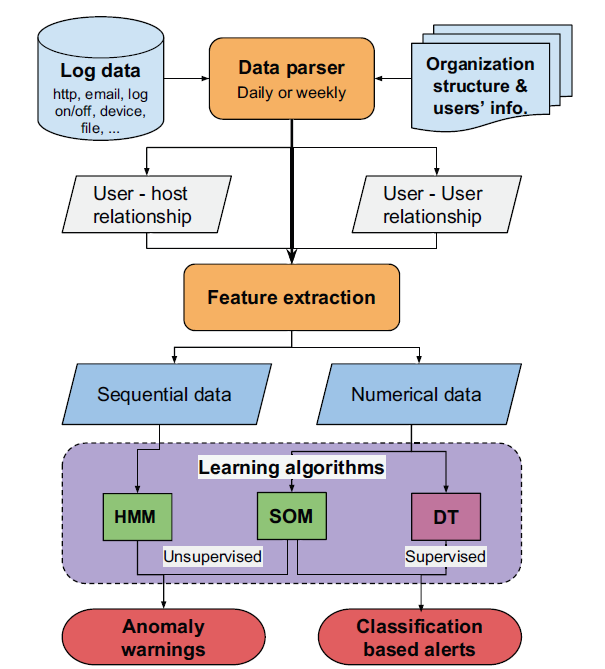
\includegraphics[height=90mm]{workflowIntrusionThreat.png}
\caption{Workflow Intrusion Threat} 
\end{figure}
\newpage
\subsection{Workflow: Learning Algorithms}

Prendiamo in considerazioni 3 algoritmi: Self-Organizing Map, Hidden Markov Model e Decision Tree; sviluppati per apprendere e modellare i dati per rilevare anomalie/minacce interne. L’obiettivo è di valutare sia gli algoritmi di apprendimento supervisionati e non.\\
Gli algoritmi di apprendimento supervisionati sono adatti per analizzare i dati con basi di veritá mentre gli algoritmi non supervisionati sono efficaci per generare avvertimenti di attivitá anomale.\\
\\
\textit{Self-Organizing Map}\\
\\

\newglossaryentry{Markov}{name={Catena di Markov},description={Una catena di markov(finita) é un sistema dotato di un numero finito di stati $\{ 1,2, .. ,n \}$ in cui la probabilità che il sistema passi dallo stato $i$ allo stato $j$ al tempo $k - 1$ é $p_{ij}(k)$}}

SOM è un un algoritmo non supervisionato basato sulle rete neurali; produce una proiezioni di dati non lineare e ordinata da un input preso in spazio multidimensionale.\\
Il SOM è costituito da una rete di neuroni artificiali i cui pesi sono continuamente adattati ai vettori presentati in ingresso nel relativo insieme di addestramento.\\
La rete neurale descritta come un insieme di neuroni artificali, ciascuno con un precisa collocazione e adiacenti gli uni dagli altri sulla mappa rappresentativa degli output, seguendo un processo dove il nodo avente un vettore di pesi piú vicino a quello dell’input si aggiudica i restanti, mentre i restanti son aggiornati in modo da avvicinarli al vettore in ingresso.\\
Quando un nodo vince una competizione, i pesi dei nodi adiacenti dove la piú un modo è lontano dal cosidetto “vincitore” meno deve essere evidente la sua variazione dei pesi.\\
Il processo viene ripetuto per ogni vettore dell’insieme di training per un certo numero di cicli, la mappa cosi riesce ad associare i nodi d’uscita con gruppi e/o schemi ricorrenti nell’insieme di dati in ingresso.\\
Vengono valutati 2 tipi di approcci per addestrare il SOM: i dati che rappresentono tutte le classi (minacce interne/esterne) altrimenti solo i dati che rappresentano i normali comportamenti dell’utente.\\
Il primo approccio è applicabile con delle ``verita di base" per dati provenienti da piú classi sono disponibili, e la veritá[ground-truth] di base vengono usate per etichettare i nodi in fase post-addestramento in base alle migliori unitá corrispondenti(nodi) per i dati in ciascuna classe.\\
Nel secondo caso quando la base di verita per una classe, tipicamente normale è disponibile per l’addestramento, il secondo approccio puó essere usato per modellare i dati ed in questo caso viene usato un rilevatore di anomalie post addestramento.\\
Quando non ci sono informazioni sui dati di addestramento, tutti i dati possono essere usati, l’obiettivo del SOM , in questo caso, è la fase di raggruppamento e visualizzazione dei dati per assistere l’analista umano.\\
\\
\textit{Hidden \Gls{Markov} Model}\\
\\ 
HMM è un modello statistico nei quali gli stati sono nascosti. Ogni stato nascosto espone un simbolo in un insieme con probabilitá prima di passare a un nuovo stato.\\
Un modello di Markov Nascosto è una \Gls{Markov} di markov dove gli stati non sono direttamente osservabili direttamente: la catena ha un certo numero di stati, gli stati evolvono secondo una Catena di Markov, ogni stato genera un evento con un certa distribuzione di probabilitá che dipende solo dallo stato, l’evento è osservabile lo stato no.\\
Possiamo usare il HMM usare l’algoritmo di Baum-Welch che data una sequenza dell’uscita o un insieme di tali sequenze, l’obiettivo è di trovare l’insieme piú probabile per il quale si possano dichiarare le probabilitá dell’uscita e di transizione.\\
Ció avviene addestrando i parametri dell’HMM mediante il gruppo di dati relativi alle sequenze di azioni di ciascun utente in un determinato periodo di tempo, in questo caso: settimanalmente.\\
Quindi, per ciascuna nuova sequenza di azioni dell'utente, l'HMM dell'utente viene utilizzato per calcolare la probabilità di log della sequenza.La sequenza viene segnalata se il valore di probabilitá di log è superiore a una certa soglia, se la sequenza non viene flaggata oppure viene considerata da un analista “non rilevante” viene usata nella combinazione con le azioni precedenti per addestrare il modello HMM dell’utente.\\
\\
\textit{Decision Tree}\\
\\
Un albero di decisione è un modello predittivo, dove ogni nodo rappresenta uno stato mentre ogni arco una determinata proprietá che porterá ad uno stato differente.\\
Per generare questo albero delle decisioni viene usato l’algoritmo C4.5, esso si basa sul costruire un decision tree usando il concetto di informazione entropica creando per ogni nodo una regola “if-then-else”.\\
Per ogni nodo dell’albero, i dati vengono suddivisi in sottoinsiemi; il criterio è soddisfatto piu efficacemente scegliendo la funzione e il punto di divisione che fornisce il massimo guadagno di informazioni normalizzate.\\
\\
\textit{C4.5}\\
\\
L’algoritmo C4.5 ha l’obiettivo di costruire un  albero decisionale da un insieme di dati di addestramento, usando il concetto di informazione entropica.\\
Essendo S un insieme di addestramento $$ S = S_1 ,S_2,…,S_n$$  di campioni gia classificati, ogni campione $s_i$ è composto da un vettore p-dimensionale $(x_{(1,i)}  ,x_{(2,i)}, … , x_{(n,i)} )$ , che rappresentano gli attributi del campione nonché le classi di cui esso appartiene.\\
L’algoritmo sceglie l’attributo che piu efficacemente divide l’insieme in piu sottoinsiemi arricchiti in una classe o in un’altra.\\
Il criterio di divisione è basato sul concetto di informazione entropica, ottenere il massimo guadagno di informazione normalizzato; l’attributo con un alto guadagno di informazioni normalizzate è scelto per creare la divisione. C4.5 è ricorsivo sulle sottoliste partizionate.
\\
\end{document}
